\documentclass[11pt,a4paper]{article}
\usepackage[
    left=0.73in,
    right=0.73in,
    top=.8in,
    bottom=.50in,
    paperheight=11in,
    paperwidth=8.5in
]{geometry}

\usepackage{array}
\newcolumntype{C}[1]{>{\centering\let\newline\\\arraybackslash\hspace{0pt}}m{#1}}

\usepackage{graphicx}
\usepackage{float}

\begin{document}
% Cover Page
\pagenumbering{gobble}
\begin{center}
\textbf{
    \Large{ECE 543: Introduction to Digital Systems}
    \\~\\
    \large{Instructor: Bessam Zuhair Al Jewad, Ph.D.}
    \\[1.25in]
    \LARGE{Prelab \#3: The Universal Logic Gate}
    \\[0.62in]
    \large{Prepared for Himadri Basu (TA)\\~\\By Christopher Chin}
    \\[1.25in]
    \LARGE{Section 6}
    \\[1.25in]
    \Large{Department of Electrical and Computer Engineering\\
           University of New Hampshire}
    \\[1.25in]
    \Large{\today}
}
\end{center}
\clearpage
\pagenumbering{arabic}

% TOC
\tableofcontents
\pagebreak

% Pages
\section{Introduction}
The objective of this experiment is to become familiar with logic gates, particularly
the NAND gate. This gate can be used to implement the six basic logic functions.

\section{Equipment Required}
\begin{itemize}
    \item Global Specialties Design and Prototyping PB-505
    \item Wire leads
    \item 7400 TTL Integrated Circuit (1)
\end{itemize}

\section{Procedure}
\subsection{IC Diagrams}
\begin{figure}[h]
    \centering
    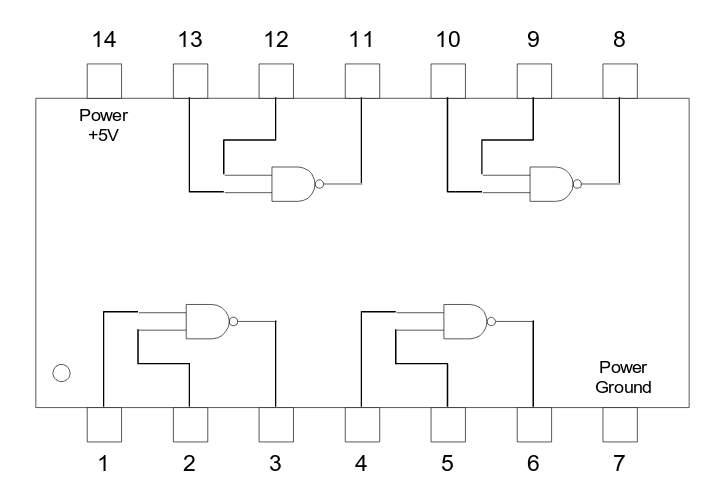
\includegraphics[width=5in]{IC.png}
    \caption{IC7400 Circuit Diagram}
\end{figure}7400
All internal gates are NAND gates.
Pin 14 is used as VCC$_{in}$. Pin 7 is GND.
Pin 1 and 2 are inputs to a logic gate that outputs to pin 3.
Pin 4 and 5 are inputs to a logic gate that outputs to pin 6.
Pin 13 and 12 are inputs to a logic gate that outputs to pin 11.
Pin 10 and 9 are inputs to a logic gate that outputs to pin 8.

\subsection{Wiring Diagrams}
\begin{enumerate}
    \item
        Basic NAND gate
        \begin{figure}[H]
            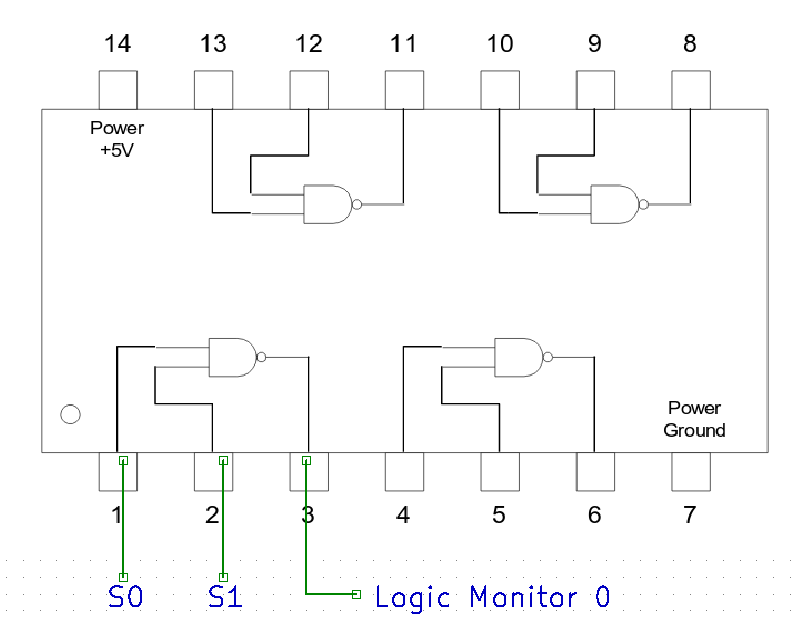
\includegraphics[width=3in]{B1.png}
        \end{figure}
    \item
        \begin{figure}[H]
            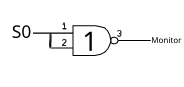
\includegraphics[width=3.3in]{B2.png}
        \end{figure}
    \item
        \begin{figure}[H]
            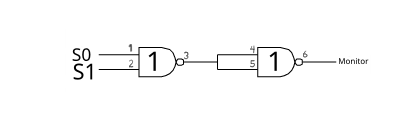
\includegraphics[width=4in]{B3.png}
        \end{figure}
    \item
        \begin{figure}[H]
            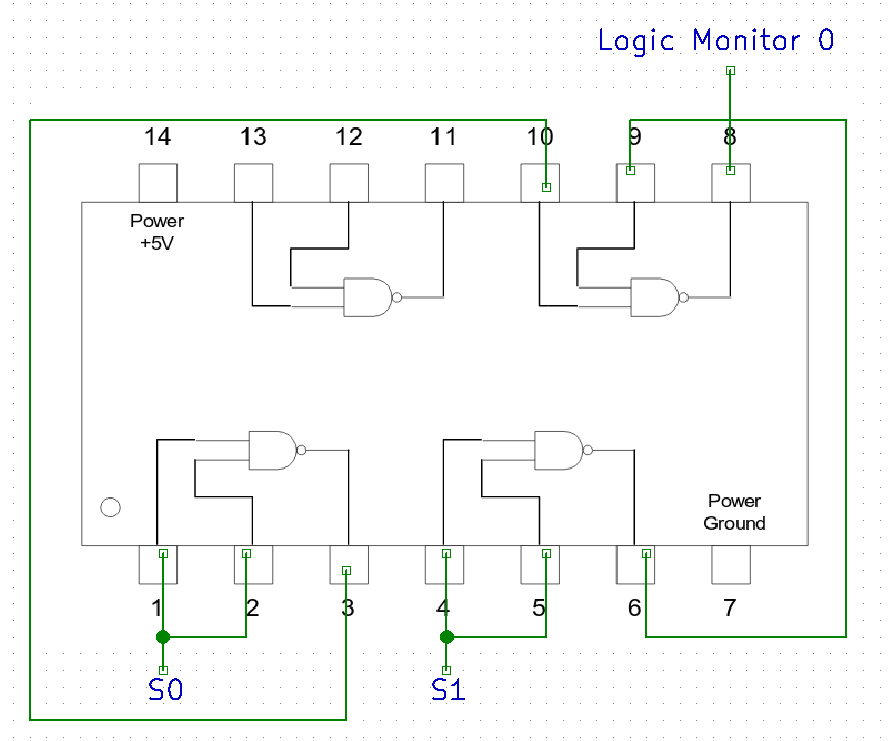
\includegraphics[width=4.2in]{B4.png}
        \end{figure}
    \item
        \begin{figure}[H]
            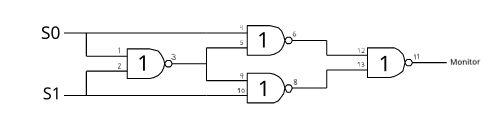
\includegraphics[width=5in]{B5.png}
        \end{figure}
    \item
        \begin{figure}[H]
            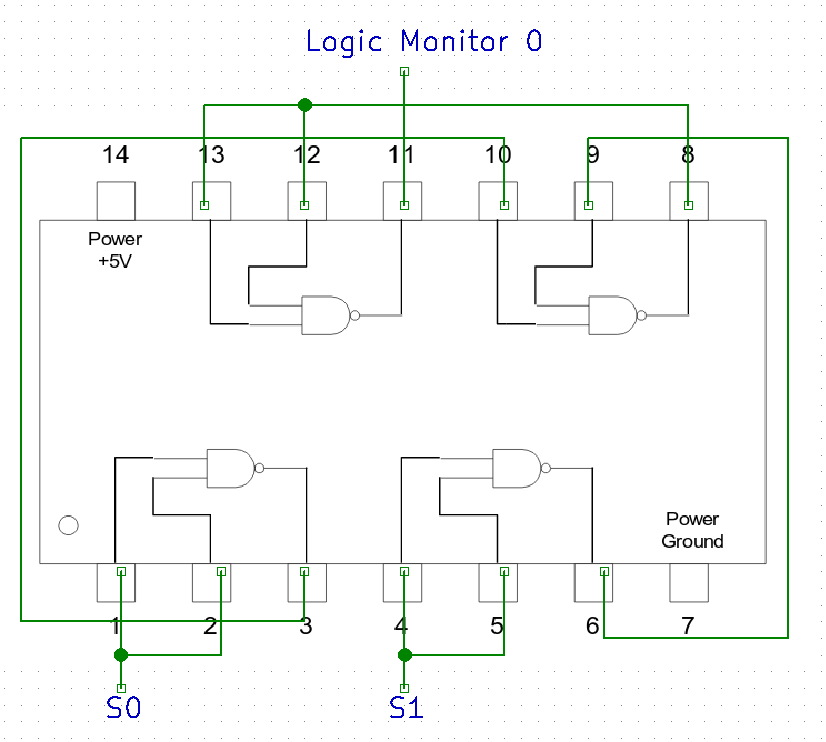
\includegraphics[width=5in]{B6.png}
        \end{figure}
\end{enumerate}
\subsection{Logic Tables}
\begin{enumerate}
    \item
        \begin{tabular}{| C{1.83cm} | C{1.83cm} | C{1.83cm} |}
            \hline
                \multicolumn{2}{|c|}{Inputs} & Output \\
            \hline S1 & S0 & Logic Monitor \\
            \hline 0  & 0  &  1 \\
            \hline 0  & 1  &  1 \\
            \hline 1  & 0  &  1 \\
            \hline 1  & 1  &  0 \\
            \hline
        \end{tabular}
    \item
        \begin{tabular}{| C{1.83cm} | C{1.83cm} |}
            \hline Input & Output \\
            \hline S0 & Logic Monitor \\
            \hline 0  & 1 \\
            \hline 1  & 0 \\
            \hline
        \end{tabular}
    \item
        \begin{tabular}{| C{1.83cm} | C{1.83cm} | C{1.83cm} | C{1.83cm} |}
            \hline
                \multicolumn{2}{|c|}{Inputs} & Intermediate & Output \\
            \hline S1 & S0 & Chip 1, Pin 3 & Logic Monitor \\
            \hline 0 & 0 & 1 & 0 \\
            \hline 0 & 1 & 1 & 0 \\
            \hline 1 & 0 & 1 & 0 \\
            \hline 1 & 1 & 0 & 1\\
            \hline
        \end{tabular}
    \item
        \begin{tabular}{| C{1.83cm} | C{1.83cm} | C{1.83cm} | C{1.83cm} | C{1.83cm} |}
            \hline
                \multicolumn{2}{|c|}{Inputs} &
                \multicolumn{2}{|c|}{Intermediates} &
                Output \\
            \hline S1 & S0 & Chip 1, Pin 3 & Chip 1, Pin 6 & Logic Monitor \\
            \hline 0 & 0 & 1 & 1 & 0\\
            \hline 0 & 1 & 0 & 1 & 1\\
            \hline 1 & 0 & 1 & 0 & 1\\
            \hline 1 & 1 & 0 & 0 & 1\\
            \hline
        \end{tabular}
    \item
        \begin{tabular}{| C{1.83cm} | C{1.83cm} | C{1.83cm} | C{1.83cm} | C{1.83cm} | C{1.83cm} |}
            \hline
                \multicolumn{2}{|c|}{Inputs} &
                \multicolumn{3}{|c|}{Intermediates} &
                Output \\
            \hline S1 & S0 & Chip 1, Pin 3 & Chip 1, Pin 6 & Chip 1, Pin 8 & Logic Monitor \\
            \hline 0 & 0 & 1 & 1 & 1 & 0\\
            \hline 0 & 1 & 1 & 0 & 1 & 1\\
            \hline 1 & 0 & 1 & 1 & 0 & 1\\
            \hline 1 & 1 & 0 & 1 & 1 & 0\\
            \hline
        \end{tabular}
    \item
        \begin{tabular}{| C{1.83cm} | C{1.83cm} | C{1.83cm} | C{1.83cm} | C{1.83cm} | C{1.83cm} |}
            \hline
                \multicolumn{2}{|c|}{Inputs} &
                \multicolumn{3}{|c|}{Intermediates} &
                Output \\
            \hline S1 & S0 & Chip 1, Pin 3 & Chip 1, Pin 6 & Chip 1, Pin 8 & Logic Monitor \\
            \hline 0 & 0 & 1 & 1 & 0 & 1\\
            \hline 0 & 1 & 0 & 1 & 1 & 0\\
            \hline 1 & 0 & 1 & 0 & 1 & 0\\
            \hline 1 & 1 & 0 & 0 & 1 & 0\\
            \hline
        \end{tabular}
\end{enumerate}
\subsection{Predictions}
Wiring Diagram Prediction
\begin{enumerate}
    \item NAND
    \item NOT
    \item AND
    \item OR
    \item XOR
    \item NOR
\end{enumerate}
Z output prediction

\begin{tabular}{| C{1.83cm} | C{1.83cm} | C{1.83cm} | C{1.83cm} |}
    \hline A & i & ii & iii \\
    \hline 0 & 1 & 0 & 0 \\
    \hline 1 & 0 & 1 & 1 \\
    \hline
\end{tabular}
\section{References}
Ronald J. Tocci et al. 2011. Digital Systems: Principles and Applications, 11\textsuperscript{th} Ed.

\end{document}
